\chapter{Requirements specification}
\textit{The requirements specification is focused around the central data uni and the sensor node. It describes the functionality requirements along with other general requirements.}
\section{General description}
The system comprises a Central data unit(CDU) and an arbitrary number of sensor nodes. The CDU serves as the main component which have several main functionalities:
\begin{itemize}
	\item Contact all sensor node within fixed time intervals
	\item Store the data locally
	\item Evaluate data and warn patient if necessary
	\item Send data to PC for analysis
\end{itemize}
The CDU supplies a bus where all sensor nodes are interconnected in a daisy chain.
The CDU continuously request measurement data from each sensor node via the bus. The CDU will be powered by a rechargeable battery with enough power to run the system for atleast a day.\\
The data should be extractable from the CDU to a PC. The connection could be bluetooth, wireless, USB, UART or some other fourth option.\\
The system is shown on figure \ref{fig:project_system} below. The focus of the requirement specification will be upon the elements shown in this figure.
\begin{figure}[H]
	\centering
	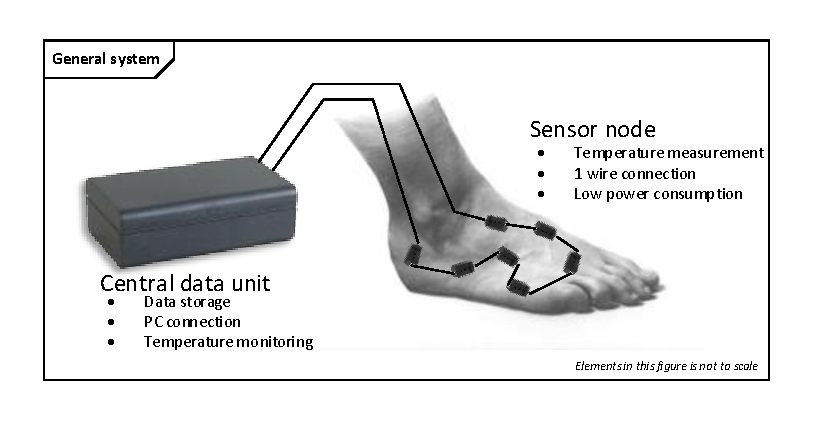
\includegraphics[width=.9\textwidth]{billeder/7requirementspec/GeneralSystem}
	\caption{Project system}
	\label{fig:project_system}
\end{figure}
The system will be mounted on and around the foot of a person who is likely to develop charcot foot. 
\section{Functionality requirements}
The system has two main functionalities:
\begin{enumerate}
	\item Set system to normal operation
	\item Extract data from CDU
\end{enumerate}
These use cases handles the expected normal functionality as seen from the end user. The users/actors of the system can be found in table \ref{tab:actors}.
\begin{table}[H]
	\centering
	\begin{tabular}{|l|l|p{9.5cm}|}
	\hline
	Actor name & Type & Description \\ \hline
	Patient & Primary & The patient sets the system to run and initiates data extraction from the CDU. \\ \hline
	Computer & Secondary  & The computer can extract data from the Central data unit. It is not intended as a control unit but mostly just for demonstration and debug purposes.\\ \hline
	\end{tabular}
	\caption{Actors of the system}
	\label{tab:actors}
\end{table}
The use case set system to normal operation has the responsibility to power on the system and set it to normal operation mode. It is initiated by the patient actor.\\
The use case extract data from CDU has the responsibility to move the stored data from the CDU to a piece of computer software. It is initiated by the patient actor and has a computer as the secondary actor. 
\begin{figure}[H]
	\centering
	\includegraphics[width=.7\textwidth]{billeder/7requirementspec/usecase_vector}
	\caption{Use case diagram}
\end{figure}
For the use cases procedures see the requirements specification document which can be found on the CD \cite{cd}.
\section{General requirements}
The requirements stated in the specifications seeks to be non-contricting to avoid restricting design opportunities.
\subsection{Functionality requirements}
\begin{table}[H]
\begin{tabular}{p{8cm} p{2cm}}
$\bullet$ Cycle: & 1 min\\
\end{tabular}
\end{table}
A cycle must include collecting data from every sensor connected to the bus. This can also be understood as the CDU must collect the overall temperature or other data every minute.\\
The data must be saved to memory which leads to the following requirement:
\begin{table}[H]
\begin{tabular}{p{8cm} p{5cm}}
$\bullet$ Memory: & 24 hours of data collection ($\sim$152kB) 256kB suggested.\\
$\bullet$ Real time clock: & Yes\\
$\bullet$ Save entries must contain: &Sensor identifier. \\
~ 									&Temperature. \\
~									&Timestamp. \\
~									&Type. \\
~									&Errors. \\
\end{tabular}
\end{table}
A real time clock must be used in order to acquire the timestamp needed in the save entries. The type of the sensor should hard coded into the device.
\subsection{Power consumption}
In order to comply with the original idea of the system, a demand for low power consumption has been made. The power consumption requirements are based on rough estimates made by the group. The power consumption requirements are as follows:
\begin{table}[H]
	\begin{tabular}{p{8cm} p{2cm}}
	$\bullet$ CDU Power consumption: & <0.5W\\
	$\bullet$ Sensor node Power consumption: & <0.05W\\
	\end{tabular}
\end{table}
The CDU power consumption requirement is excluding the sensor node power consumption.
\subsection{Interface requirements}
In the central data unit requirements part of the general requirement section in the requirements specification document it is stated that the system interfaces must be:
\begin{table}[H]
	\begin{tabular}{p{8cm} p{2cm}}
	$\bullet$ Custom power line communication bus: & Yes\\
	$\bullet$ CDU to computer interface: & Yes\\
	\end{tabular}
\end{table}
The sensor nodes require the Custom power line communication bus as a system interface as well.
%\subsection{Other requirements}
%A BOM (Build of Materials) price have been specified in the requirements. The original project formulation specifies a need for minimising the production cost. The price is rather high as it serves as food for thought. The production price still has unknown elements like assembly cost which is why a materials price have been specified.